\documentclass[12pt]{article}%
\usepackage{amsfonts}
\usepackage{fancyhdr}
\usepackage{comment}
\usepackage[a4paper, top=2.5cm, bottom=2.5cm, left=2.2cm, right=2.2cm]%
{geometry}
\usepackage{times}
\usepackage{amsmath}
\usepackage{changepage}
\usepackage{amssymb}
\usepackage{graphicx}
\usepackage{diagbox}
%
\setcounter{MaxMatrixCols}{30}
\newtheorem{theorem}{Theorem}
\newtheorem{acknowledgement}[theorem]{Acknowledgement}
\newtheorem{algorithm}[theorem]{Algorithm}
\newtheorem{axiom}{Axiom}
\newtheorem{case}[theorem]{Case}
\newtheorem{claim}[theorem]{Claim}
\newtheorem{conclusion}[theorem]{Conclusion}
\newtheorem{condition}[theorem]{Condition}
\newtheorem{conjecture}[theorem]{Conjecture}
\newtheorem{corollary}[theorem]{Corollary}
\newtheorem{criterion}[theorem]{Criterion}
\newtheorem{definition}[theorem]{Definition}
\newtheorem{example}[theorem]{Example}
\newtheorem{exercise}[theorem]{Exercise}
\newtheorem{lemma}[theorem]{Lemma}
\newtheorem{notation}[theorem]{Notation}
\newtheorem{problem}[theorem]{Problem}
\newtheorem{proposition}[theorem]{Proposition}
\newtheorem{remark}[theorem]{Remark}
\newtheorem{solution}[theorem]{Solution}
\newtheorem{summary}[theorem]{Summary}
\newenvironment{proof}[1][Proof]{\textbf{#1.} }{\ \rule{0.5em}{0.5em}}

\newcommand{\Q}{\mathbb{Q}}
\newcommand{\R}{\mathbb{R}}
\newcommand{\C}{\mathbb{C}}
\newcommand{\Z}{\mathbb{Z}}

\begin{document}

\title{Tutorial 3}
\author{Wangzhihui Mei \\ 2019124044 6603385}
\date{}
\maketitle

\section*{Exercise 1}
\begin{center}
    \begin{table}[h]
        \begin{tabular}{|l|l|l|l|l|}
            \hline
            \diagbox{State}{Input} & s & . & e & d \\ \hline
            I & B &   &   & C \\ \hline
            B &   & D &   & C \\ \hline
            C &   &   &   & C \\ \hline
            D &   &   &   & E \\ \hline
            E &   &   & F & E \\ \hline
            F & G &   &   & H \\ \hline
            G &   &   &   & H \\ \hline
            H &   &   &   & H \\ \hline
        \end{tabular}
    \end{table}
\end{center}


    
 
\section*{Exercise 2}
\begin{figure}[]
    \centering
    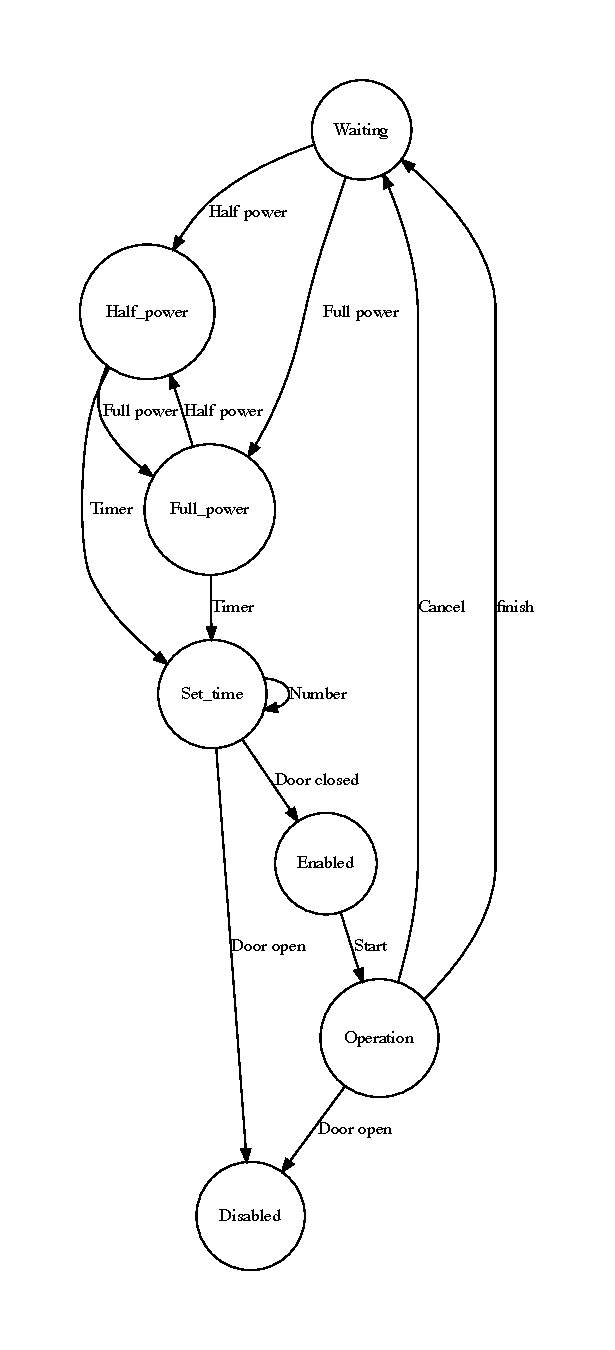
\includegraphics[]{ovenfsm}
    \caption{FSM for the oven }
\end{figure}

\end{document}